
\section{Catena Elettronica Completa}\label{sec:catena}
In questa sezione si assembla un circuito amplificatore con l'obiettivo di portare l'output dello shaper
entro i range tipici dei sistemi di acquisizione dati (DAQ), generalmente tra i $2\V$ e i $5\V$.
Essendo già positivo il segnale in uscita dallo shaper, si assembla il circuito in configurazione non invertente,
come mostrato nel terzo e ultimo modulo della catena rappresentata in Figura~\ref{fig:circ_tot}. Dopo aver calcolato gli opportuni valori delle resistenze $R_{1a}$ e $R_{2a}$,
si connette l'amplificatore al resto della catena elettronica e se ne studia la linearità e la risposta in
frequenza.

\subsection{Configurazione sperimentale e prime misure}\label{sec:catena_config}
Per capire con quali resistenze costruire il circuito, si manda in ingresso
al preamplificatore un'onda quadra di periodio $15\us$ e si registra la
tensione massima di output dello shaper $V_{\text{sh}}^{\text{max}}=0.290\pm 0.006\V$.
Data la funzione di trasferimento di un amplificatore non invertente
\begin{align}
  A(s)=1+\frac{R_{a2}}{R_{a1}}
\end{align}
segue che, per ottenere una tensione di $2\V$ in uscita dalla catena elettronica, il rapporto tra le due resistenze deve valere $R_{a2}/R_{a1}=5.9$. Con le resistenze a disposizione si sceglie
$R_{a1}=32.80\pm 0.2\kOhm$ mentre la resitenza di feedbeck si realizza mettendo in serie
due resistori di impedenza equivalente
\begin{align}
  R_{a2}= (67.9\pm 0.3)\kOhm + (120.6 \pm 0.6)\kOhm = (188.5 \pm 0.7)\kOhm
\end{align}
Si prevede quindi un'amplificazione $A=6.75\pm 0.06$, debolmente compatibile con quella richiesta ($\lambda=2.5$). Per verificare la correttezza delle ipotesi si manda in ingresso all'amplificatore invertente appena
assemblato un'onda sinusoidale di frequenza $1\kHz$ e ampiezza $1\V$ e
si misura con l'oscilloscopio la risposta del circuito. Successivamente, si
inserisce il segnale di uscita dello shaper come input dell'amplificatore non
invertente e si misura nuovamente la risposta del circuito. I valori acquisiti e le compatibilità con le aspettative teoriche vengono riportati in
Tabella~\ref{tab:amp_misure}, la quale evidenzia un'ottimo accordo e conferma quindi
la correttezza dell'apparato sperimentale.
\begin{table}[h]
\renewcommand{\arraystretch}{1.6}
\centering
\setlength{\tabcolsep}{10pt}
\begin{tabular}{ |cccc| }
\hline
\multicolumn{4}{|c|}{Preamplificatore - onda sinusoidale} \\
$V_{\inp}^{\text{max}}=0.99\pm 0.02\V$ & $V_{\out}^{\text{max}}=6.67\pm 0.12\V$ & $A_{\text{amp}}=6.8\pm 0.2$ & $ \lambda_{A}=0.14$\\
\hline
\multicolumn{4}{|c|}{Catena elettronica - onda quadra} \\
$V_{\inp}^{\text{max}}=-1.00\pm 0.02\V$ & $V_{\out}^{\text{max}}=2.08\pm 0.04\V$ &$|A_{\text{catena}}|=2.09\pm 0.06$ & $\lambda_{V_{\out}}=1.9$ \\
\hline
\end{tabular}
\caption{\footnotesize Si mostrano le misure acquisite con l'oscilloscopio in due configurazioni: onda sinusoidale in input al preamplifcatore e onda onda quadra in  ingresso alla catena completa. Si calcolano inoltre le compatibilità tra l'amplificazione prevista e quella osservata (nel primo caso) e tra la tensione in output misurata e il valore richiesto di $2\V$ (nel secondo caso).}\label{tab:amp_misure}
\end{table}
%-------------------------------------


\subsection{Analisi del circuito }\label{sec:catena_analisi}
La catena elettronica completa, mostrata in Figura~\ref{fig:circ_tot}, ha come funzione di
trasferimento il prodotto delle funzioni di trasferimento dei tre moduli che
la compongono
\begin{align}
  A(s)= A_{\text{pre}}(s) \, A_{\text{sh}}(s) \, A_{\text{ampl}}(s) = \left(-
  \frac{\frac{1}{R_{1}C_{\text{f}}}}{s+\frac{1}{\tau_{\text{pre}}}}\right) \, \left(\frac{1}{\tau_{\text{sh}}}\,\frac{s+\frac{1}{\tau_{\text{pz}}}}{(s+\frac{1}{\tau_{\text{sh}}})(s+\frac{1}{\tau_{\parallel}})}\right) \,\left(1+\frac{R_{a2}}{R_{a1}}\right)
\end{align}
Avendo scelto la resistenza $R_{\text{pz}}$ tale che $\tau_{\text{pz}} = \tau_{\text{pre}}$ ed essendo essa molto più grande delle resitenze dello shaper la funzione di trasferimento assume la forma semplificata
\begin{align}
  A(s)=- \frac{1}{R_{1}\,C_{\text{f}}\, \tau_{\text{sh}}} \,\,
  \frac{1+\frac{R_{2a}}{R_{1a}}}{\left(s+\frac{1}{\tau_{\text{sh}}}\right)^{2}}
\end{align}
La funzione di trasferimento è quindi caratterizzata dall'assenza di zeri e
dalla presenza dello stesso polo doppio trovato nello shaper. La catena si comporta
quindi come un filtro passa basso: per frequenze piccole il grafico di Bode presenterà un andamento costante, mentre per frequenze elevate si prevede
una decrescita lineare di $40\,dB/dec$. La frequenza di taglio attesa è la
stessa calcolata nella Sezione~\ref{sec:shaper_bode_analisi}, ovvero $f_{t}= 15.5\pm 0.2\kHz$.

\subsection{Linearità della Catena Elettronica}\label{sec:catena_lin}
Si vuole ora verificare la linearità del massimo del segnale di uscita $V_{\out}^{\text{max}}$ della catena elettronica rispetto alla quantità di carica iniettata nel preamplificatore $Q_{\text{in}}$. Si modifica quindi la
durata dell'impulso del generatore tra $5\us$ e $15\us$ e si misura con
l'oscilloscopio il massimo del segnale rilevato.

\subsubsection{Analisi dati }\label{sec:catena_lin_analisi}
Per l'analisi dati si procede esattamente come in Sezione~\ref{sec:preamp_lin}: si calcola la
quantità di carica $Q_{\inp}$ per ogni valore di $T$ utilizzato e, a causa
della correlazione totale degli errori sulle cariche, si effettua il fit senza prendere in considerazione gli errori sulle ordinate. A differenza di
quanto svolto in precedenza però, si sceglie di non correggere l'errore sulla pendenza effettuando un primo fit rispetto ai periodi. In questa sezione si preferisce infatti concetrarsi solo sulla verifica della linearità e quindi
sul grafico dei residui, che non è influenzato dalla presenza di errori di
scala costanti. I risultati del fit vengono mostrati in Figura~\ref{fig:catena_fit_lin}, che evidenzia una buona distribuzione dei residui attorno allo zero e una leggera
sovrastima degli errori per i periodi più grandi. Il chi quadro presenta un'ottima
compatibilità col valore atteso ($\lambda=0.11$). Si conferma quindi l'ipotesi di linearità
della catena elettronica.
%------------------------------------
\begin{figure}[h]
\centering
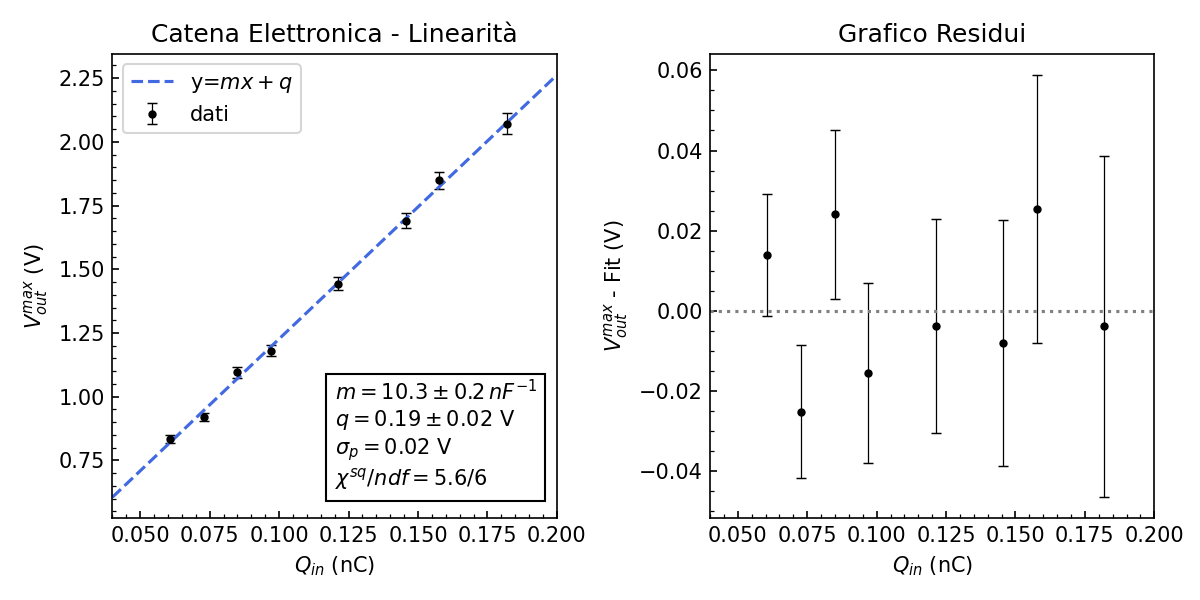
\includegraphics[width=1\textwidth]{../ampli/images/fit_lin}
\caption{\footnotesize A sinistra si mostrano le coppie $(V_{\text{out}}^{\text{max}}, Q_{\text{in}})_{i}$ e la retta interpolante. A destra, viene riportato il grafico dei residui.}\label{fig:catena_fit_lin}
\end{figure}
%------------------------------------

\subsection{Risposta in frequenza della Catena Elettronica}\label{sec:catena_bode}
Si vuole infine approfondire la risposta in frequenza della catena elettronica. Si acquisce quindi il massimo della tensione in uscita $V_{\out}^{\text{max}}$
per segnali sinusoidali di frequenza variabile tra $10 \Hz$ e $100\kHz$. Si rappresentano quindi i dati in un grafico di Bode e si stima la frequenza di taglio della catena a partire da due interpolazioni lineari.

\subsubsection{Analisi dati }\label{sec:catena_bode_analisi}

Il grafico di Bode mostrato in Figura~\ref{fig:catena_fit_bode} viene realizzato calcolando la
funzione di trasferimento in Decibel, come spiegato nella Sezione~\ref{sec:preamp_bode}.
I dati vengono inoltre confrontati con una simulazione, che evidenzia un ragionevole accordo con le misure sperimentali, in particolare per basse frequenze. Si osserva inoltre l'andamento
previsto in Sezione~\ref{sec:catena_analisi}: inizialmente la funzione di trasferimento
è approssimabile ad una retta di pendenza nulla ($m_{1}=0.10\pm 0.04\, dB/dec$) mentre a frequenze
più elevate si ha una decrescita linare ($m_{2}=-34.0\pm 0.5\, dB/dec$) che tuttavia risulta incompatibile all'aspettativa teorica di $-40 \,dB/dec$. Per
alte frequenze infatti, si inizia ad osservare un leggero discostamento rispetto alla simulazione attribuibile alla non idealità degli elementi
che compongono il circuito.
Dall'intersezione delle due rette si stima infine la frequenza
di taglio $f_{t,\text{fit}}=12.4\pm 0.2 \kHz$, incompatibile con l'aspettativa teorica ($\lambda=9.9$) ma
in ottimo accordo con la stima ottenuta a partire dal grafico di Bode dello shaper nella Sezione~\ref{sec:shaper_bode} ($\lambda=0.1$).
%------------------------------------
\begin{figure}[h]
\centering
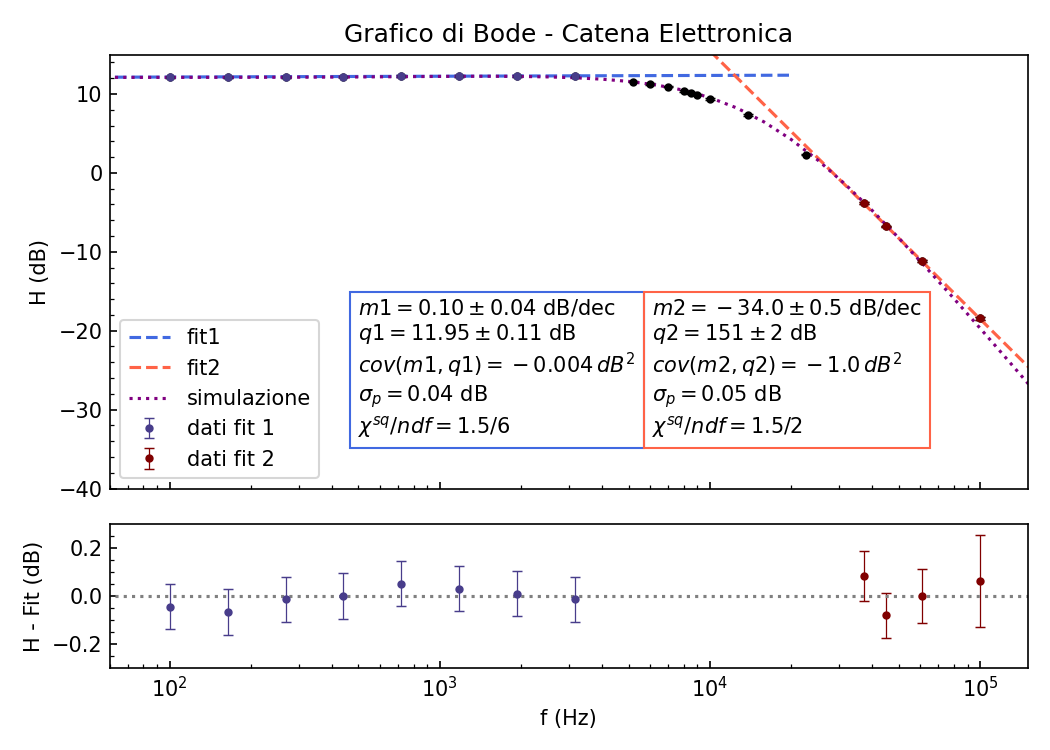
\includegraphics[width=0.8\textwidth]{../ampli/images/fit_bode}
\caption{\footnotesize{Grafico di Bode della catena elettronica completa e simulazione LTspice. Si mostrano anche i residui delle due interpolazioni da cui si è ricavata la frequenza di taglio.}}\label{fig:catena_fit_bode}
\end{figure}
%------------------------------------

\section{Conclusioni}
\label{sec:conclusioni}
La catena elettronica così prodotta permette quindi di trasformare il segnale
di corrente di un sensore di radiazione (che nel nostro caso è stato simulato da un'onda quadra in ingresso) in un segnale adatto ad un generico DAQ che lavora in un range attorno ai $2\V$. Tuttavia, analizzando singolarmente i moduli della catena, sono state osservate numerose discrepanze con le aspettative teoriche e con le simulazioni: in particolare, lo shaping time e la tensione massima prevista in output allo shaper risultano particolarmente anaomale. Conseguentemente, anche la frequenza di taglio della catena elettronica è incompatibile con quella prevista.   Questo rende il circuito realizzato non ottimale, soprattutto se confrontato a sistemi elettronici più complessi e costosi che sono in grado di gestire segnali anche piu piccoli e veloci grazie ad una banda più larga e ad una migliore gestione del rumore.
